\newpage
\section{Solution Approaches}
\hl{SECTION UNDER CONSTRUCTION}\\
Implementation with the DEAP Framework for Python \cite{DeRainville:2012}

\iffalse
\hl{Content:}
\begin{itemize}
    \item \hl{The research method by which you will investigate the world. }
        \subitem \hl{A short summary of the available methods}
        \subitem \hl{Your choice}
        \subitem \hl{Detailed report of how you actually carried out your research. Presenting how you selected the people taking part is of special importance.}

    \item \hl{The third chapter of the Master's Thesis is the Materials and Methods, sometimes also referred to as the Study Design and Methodology. It is in this section that the writer describes the sample population and procedures used in enough detail that others could replicate the study and verify its validity. This section should begin with specific data on the number of study participants, how they were chosen, and relevant demographic information. The writer may also present the rationale for the specific sample size used. Next, all tools and instruments used in the study should be described. If such tools are described in detail elsewhere in the literature, the writer can indicate this along with a relevant reference. Actual surveys or questionnaires will not be presented here. Instead, the writer provides an overview and then inserts copies of the tools into the Appendix at the end of the paper. }
\end{itemize}
\fi

\subsection{Evolutionary algorithm for the Basic Role-Mining Problem}
\hl{SECTION UNDER CONSTRUCTION}\\
    \subsubsection{Representation of individuals}
    In a first attempt I tried to represent an RBAC model as individual with a bit-string. The bit-string is derived from a combined UR- and RP-Matrix. Figure \ref{fig:representation1} shows an example. The motivation of this initial idea was that the mutation operator can be easily executed by just flipping a bit within the bit-string. However, the problem with this representation is that the number of roles needs to pre-defined.\\
    \begin{figure}[H]
        \centering
        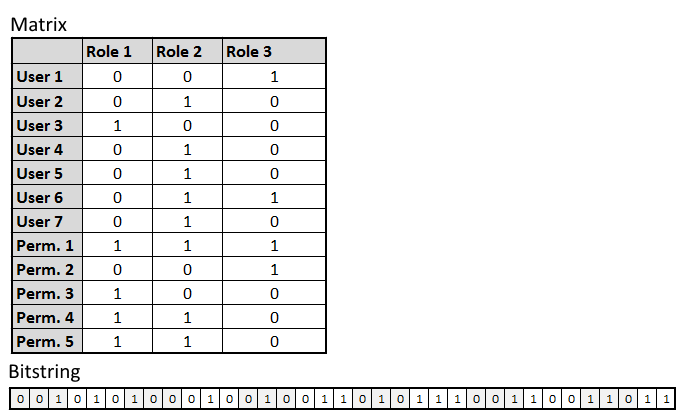
\includegraphics[scale=0.75]{./Figures/Representation1.png}
        \rule{20em}{0.5pt}
        \caption{\textit{Example of a combined UR- and RP-Matrix with its bit-string representation}}
        \label{fig:representation1}
    \end{figure}
    In \cite{saenko2012design} two different representations are introduced. In the first representation the authors suggest to build an individual out of three chromosomes X, Y and Z. Chromosome X describes the UR-Matrix, chromosome Y describes the RP-Matrix and chromosome Z is a vector, which marks roles as active or passive. With this representation the number of roles becomes part of the search. An example can be seen in figure \ref{fig:representation2}. The drawbacks of this representation are unnecessary genes (roles) and complex crossover operations\cite{saenko2012design}. The second improved representation eliminates these drawbacks by having one chromosome for an individual, where no unnecessary genes occur. The chromosome consists of a list of roles, which contain a user-set and a permission-set (see figure \ref{fig:representation3}).\\
    Due to the advantages of the last mentioned representation, this is chosen to be the representation for the research of single-objective EAs for solving the RMP.\\
    
    \hl{Description of data structure}

    \subsubsection{Initialization of the Population}
    The initial population is randomly generated by creating chromosomes (RBAC models) of random gene size (role size), which contain a random set of users and permissions. It is ensured that each role has at least one user and permission assigned.
    
    \subsubsection{Mutation methods}
    For the mutation six different mutation types are implemented, which are randomly executed.
    \begin{itemize}
        \item 1. Add a new role
        \item 2. Remove a role
        \item 3. Add a user to a role
        \item 4. Remove a user from a role
        \item 5. Add a permission to a role
        \item 6. Remove a permission from a role
    \end{itemize}
    
    \hl{Pseudocode?}
    
    \subsubsection{Crossover methods}
    The recombination is executed on two individuals with a traditional one-point crossover. In the crossover operation the roles of the parents are merged to new individuals.\\
    \hl{Pseudocode?}
    
    \subsubsection{Evaluation functions}
    Several objectives of the role mining problem are separately implemented as evaluation function and their impact on the EA is analyzed. In \cite{saenko2012design} a weighted function is suggested which takes the number of roles, access-violations and availability-violations into account. The function is formulated as maximization function. Another commonly used objective function, the weighted structural complexity, is also implemented and compared with the first function. Different weights for the functions are tested and reveal that the objective of minimizing the number of roles has a strong influence.\\
    To analyze the different objectives a MOEA has been implemented. The NSGA-II algorithm is applied and reveal the algorithm is not good in handling individuals with the same fitness. The Fortin improvement is applied. Since the objective of number of roles has a too strong impact, a NSGA-II algorithm with weights is implemented.\\
    
    \hl{Pseudocode?}
    
    \begin{itemize}
        \item NSGA2\\
        Why? The higher the role number (1 Role for each user), the more likely it is to have no violations. The lower the role number, the more violations
        \item Improved NSGA2 (Fortin)\\
        Why? Different Individuals have same fitness
        \item Weighted NSGA2\\
        Why? 2nd objective is less important\\
        Issue? Skipped fronts, no symmetry in domination matrix
    \end{itemize}
        
    \subsubsection{Selection mechanisms}
    Which selection mechanisms are chosen is dependent on if a single-objective or a multi-objective EA is applied.\\
    For the parent selection ...\\
    For the survivor selection ...\\
    DEAP Build-in selection methods\\
    Improvements of DEAP Build-in selection methods\\
    \hl{Pseudocode?}
    
\subsection{Evolutionary algorithm for the Inference Role-Mining Problem}
\hl{SECTION UNDER CONSTRUCTION}\\
\hl{Not implementation yet}

\subsection{Alternative approach with Co-Evolution}
\hl{SECTION UNDER CONSTRUCTION}\\
Instead of that individuals represent RBAC models, the individuals represent roles. The motivation behind this approach is to involve human interaction in the survival selection of the EA. Since a whole RBAC model can be hardly evaluated at once, the individuals have to be a smaller fraction of the RBAC model.

    \subsubsection{Symbiotic, Adaptive Neuro-Evolution (SANE)}

\subsection{Human interaction}
\hl{SECTION UNDER CONSTRUCTION}\\
\hl{Not implemented}
